\section{Moving Beyond Flat Index Tags} \label{sec:background}

%\begin{figure}[t!] \begin{minipage}{1\linewidth}
%\begin{subfigure}[c]{0.96\linewidth} 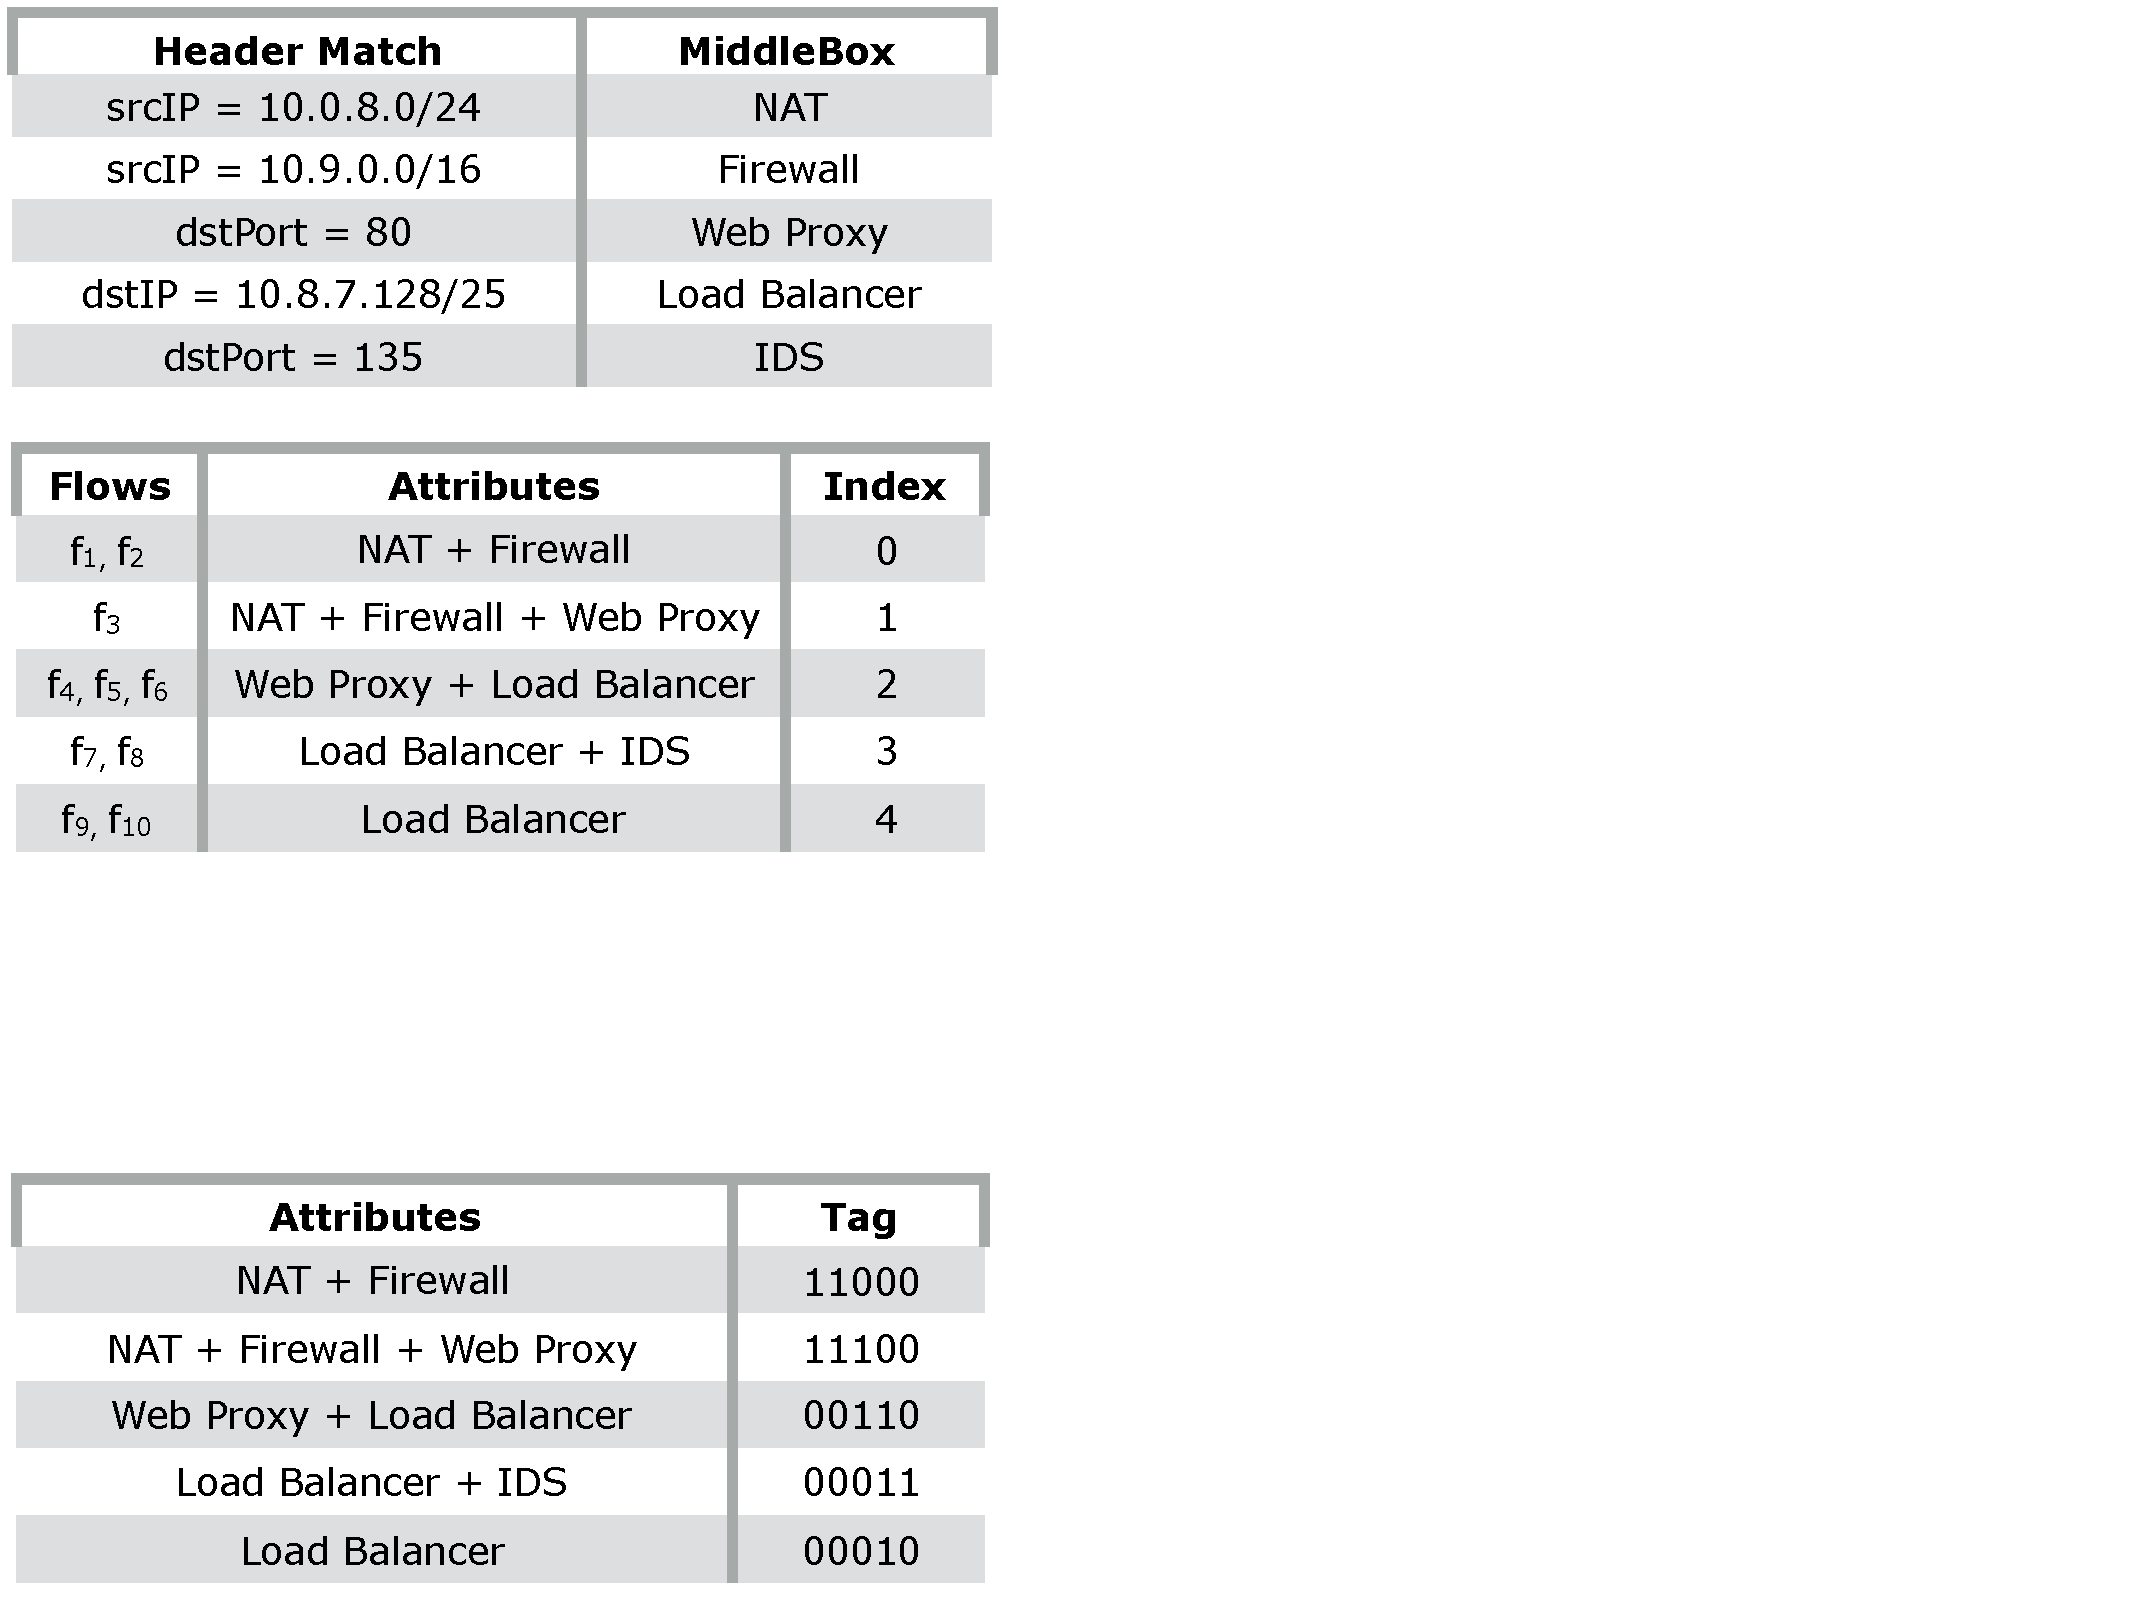
\includegraphics[trim={0 12cm 19cm 0},
%clip, width=\linewidth]{figures/mbox_path_example3} \end{subfigure}
%\end{minipage} \caption{In this example, we have a policy that defines traffic
%which must flow through subsets of five middleboxes. The first table shows
%which header fields trigger each middlebox, and the second table shows some
%combinations we may see in network traffic. } \label{fig:mbox_policies}
%\end{figure}

Packet labeling schemes need to work within the capabilities of commodity
switches.  In this section, we first review packet forwarding in high-speed
switches and how the ``match-action'' capabilities have evolved in recent years.
Next, we discuss flat index tagging and its limitations. 

\subsection{Flexible Tags using Flexible Switches} Commodity switches
traditionally use \emph{match-action tables} to determine how to handle packets,
based on \textit{forwarding rules} installed at runtime. A table entry consists
of a set of match conditions, and an action to take if the matching conditions
are met. Actions include dropping a packet, rewriting a header field, or
forwarding the packet out a specific port.  Each matching condition compares a
string $S$ to a specific packet header field $H$, using one of three kinds of
comparisons:

\begin{itemize} \item \textbf{Exact Matching:} $S$ is a binary string, and the
match returns true if $S = H$.  \item \textbf{Longest-Prefix Matching:} $S$ is a
ternary string, where the first $x$ characters are binary, and the remaining are
the wildcard character $*$. A header field is a match if the $x$ binary
characters of $S$ are a prefix of $H$, and there is no other $S'$ in the table
which is a longer prefix of $H$.  \item \textbf{Wildcard Matching:} $S$ is a
ternary string with characters $\{0,1,*\}$ and an associated priority. $S$
matches $H$ if the only characters on which they are unequal are wildcards, and
there is no other $S$ in the table which also matches but has a higher priority.
\end{itemize}
  
Until recently, switches imposed significant restrictions on the matching type.
For the vast majority of fields, only exact matching was supported, with the
exception of longest-prefix matching for IP addresses. This prevents most fields
from being repurposed for anything other than flat tags. However, with recent
changes to commodity switches, such as new features supported by OpenFlow 1.3
switches~\cite{of13} and flexible protocol-independent switches~\cite{P4}, we
can apply longest-prefix or wildcard matching to existing fields, or even add
new fields. Prefix and wildcard matching allows us to treat a header field as a
\emph{set} of information, rather than just a single value. 

\subsection{Forwarding Equivalence Class Tagging} In flat tagging schemes, the
tag serves as a single, unstructured index.  A flow of packets is defined by a
combination of header fields that each of the packets has in common. Each
combination of header fields can imply a set of attributes which are revealed by
classification, such as a set of routes the flow may take, middleboxes the flow
must traverse, or permissions of the sending/receiving hosts relevant to
security policies.  Figure ~\ref{fig:mbox_path} shows a simple example of
service chaining. Every flow is mapped to one of two paths through network nodes
by some policy, and the network must be aware of the full path to route
correctly. In our example, not all flows should traverse switch $E$. To avoid
reclassification at each node, the example shows a simple tagging scheme where
each of the two paths receives a unique index. If the switches have up to date
knowledge of which index maps to which attribute set, reading the tag determines
the next-hop. 

Index tagging is optimal in tag width, because it uses $\log_2{N}$ bits to
identify one of $N$ attribute sets. However, small tags comes at the cost of
complexity in reading the attributes. In our example, the first segment of the
path is identical for both tags, yet switches, without the ability to perform
wildcard or prefix matching, must have exact rules for every tag. In general, if
the number of tags is large enough, this flat tagging scheme may have forwarding
table entries on the order of the number of entries packet classification
requires!



\begin{figure}[t!] \begin{minipage}{1\linewidth} 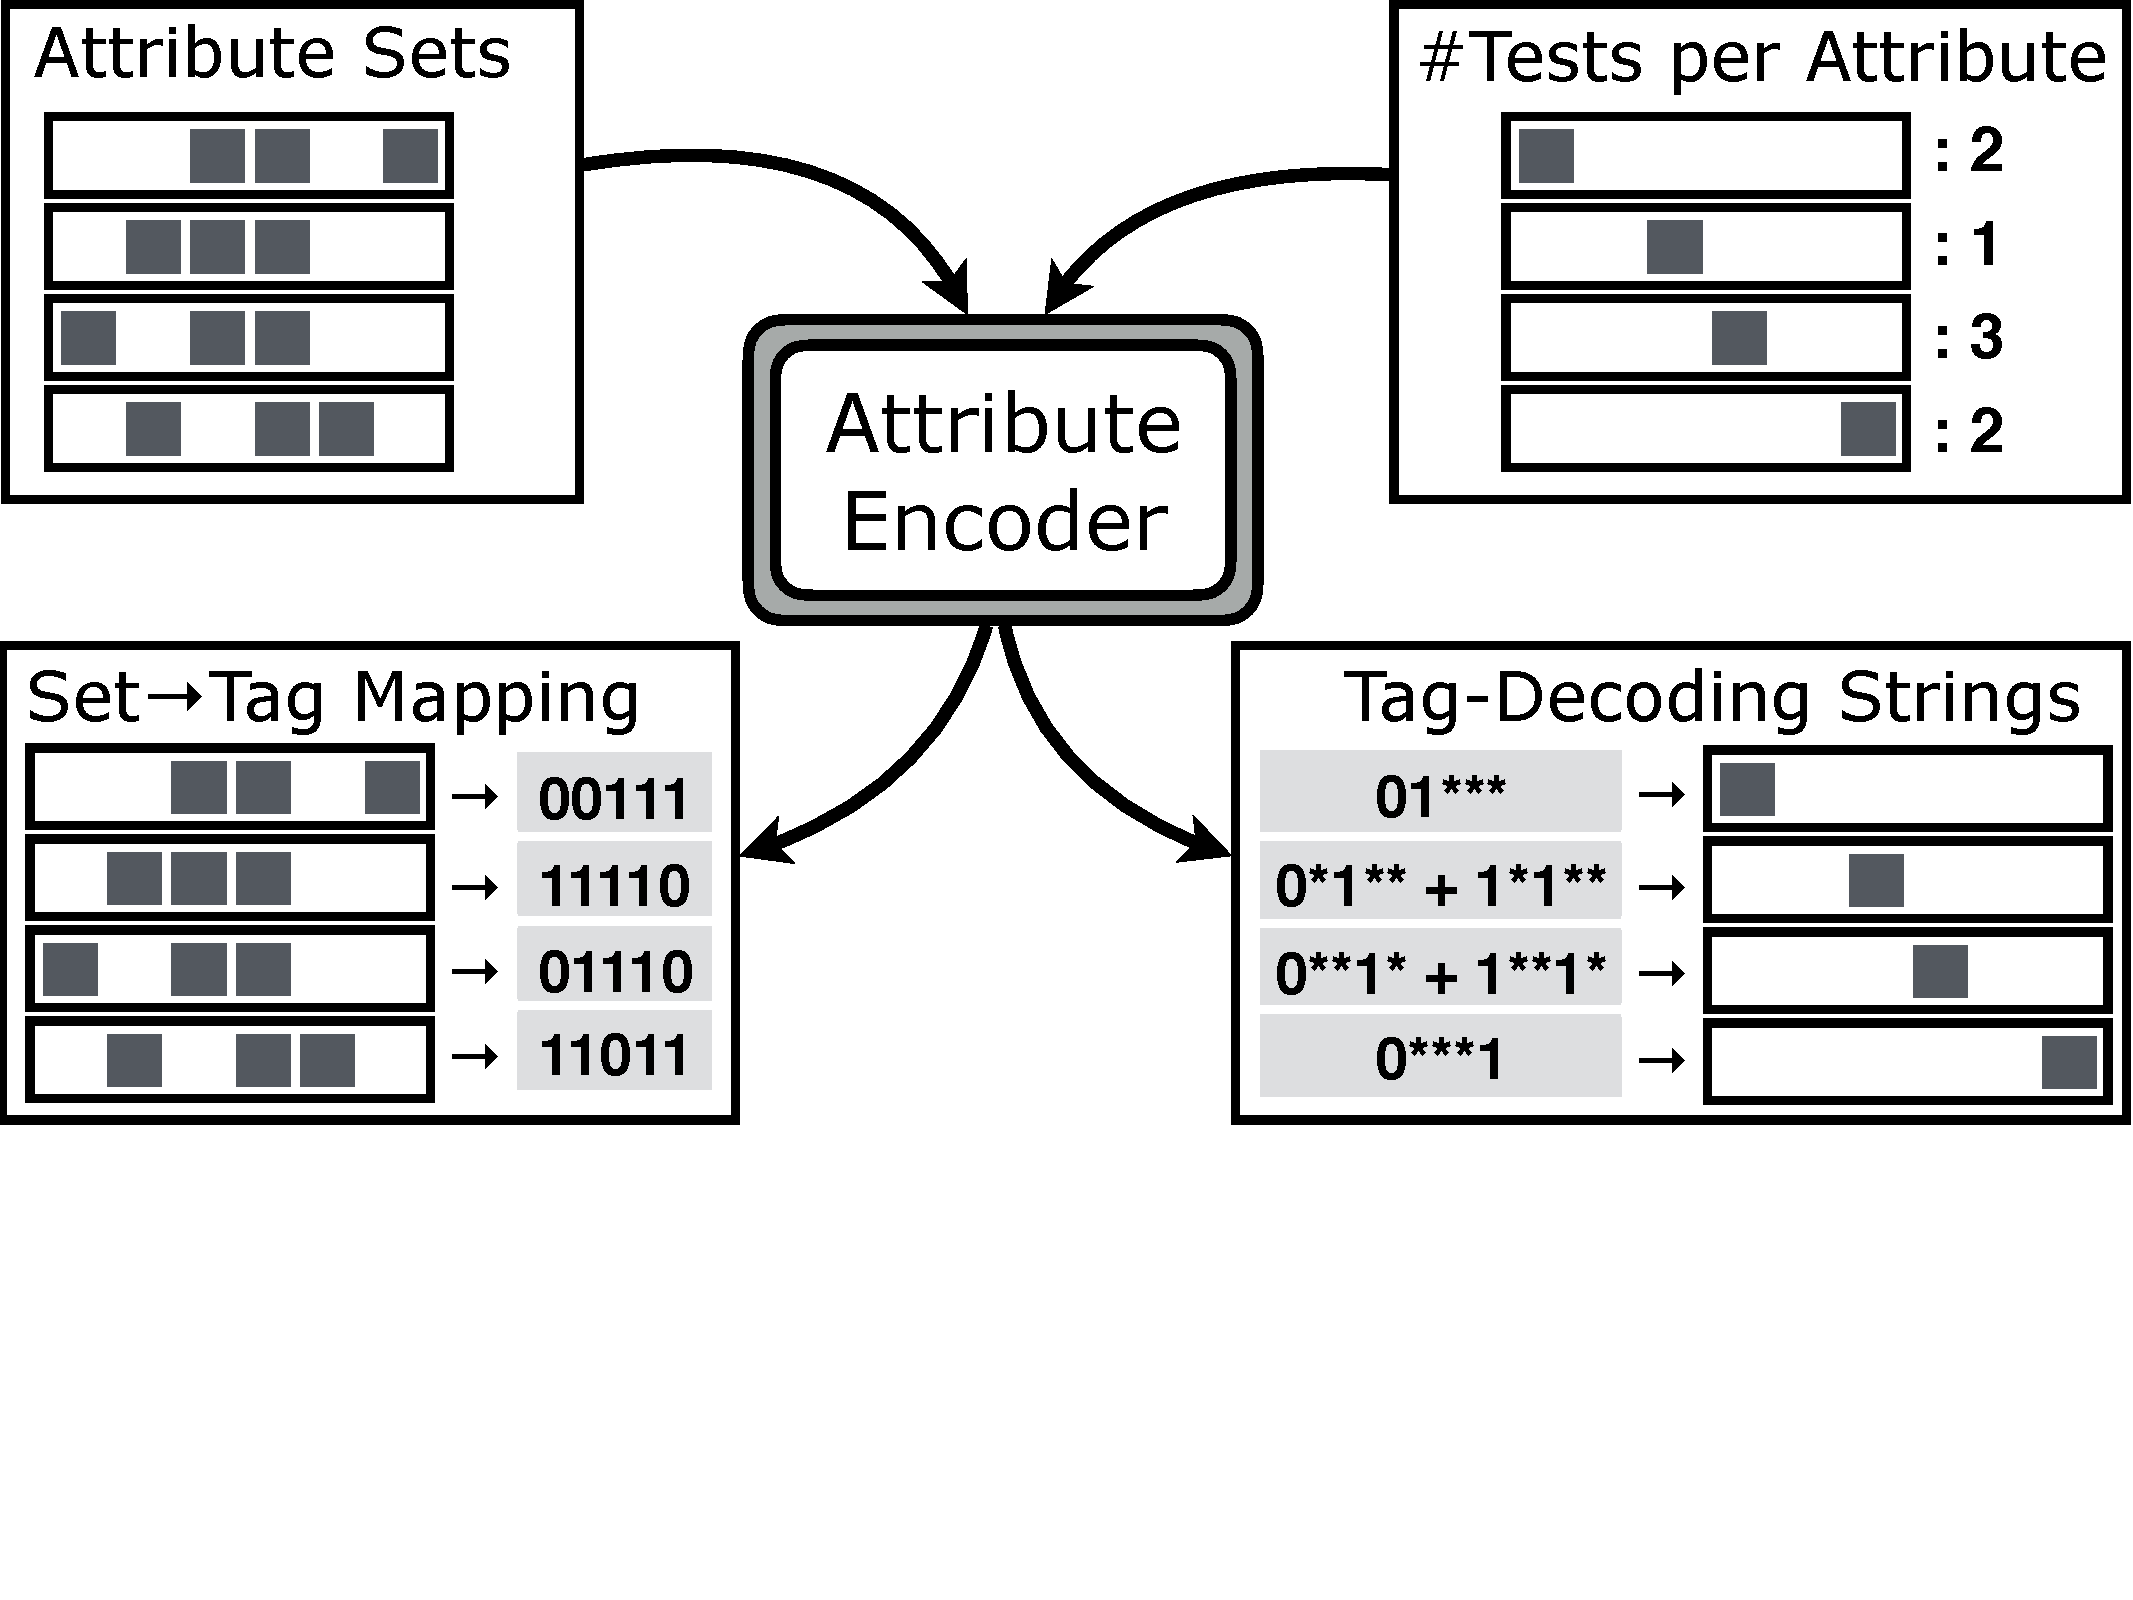
\includegraphics[trim={0 4cm 0
0}, clip, width=\linewidth]{figures/system_flow2} \end{minipage} \caption{An
illustration of the information flow for an attribute-encoding tagging scheme.
The encoding scheme takes as input a list of attribute sets and the number of
queries that will be performed per attribute. The output is a list of tags
corresponding to those attribute sets, and wildcard strings used for querying
each attribute.} \label{fig:system_flow} \end{figure}


\subsection{Strawman Bitmask Tags}

Attribute reading need not be so complex, though. If we do not require minimal
tag width, we can make the attributes much easier to read.  Assume that it is
possible to attach an arbitrarily large tag to each packet the moment it is
classified, and that network switches can perform masked matching on this tag.
We can easily use this hypothetical tag to encode and decode any attribute. If
there are $N$ possible attributes, we can write $N$ bits to the tag: the
$i^{th}$ bit corresponds to the $i^{th}$ attribute. The moment the packet is
classified, the $i^{th}$ bit is set to 1 if the $i^{th}$ attribute is present
for that flow, and 0 if it is not. As a result, if we wish to test for the
    presence of attribute $x$, we need only check that $x$'s bit is 1 in the
    metadata before rerouting, rather than exact matching on every tag that
    contains $x$.

Of course, we cannot attach arbitrary metadata to packets. Rather, we can
repurpose a field in the header for tagging. In FlowTags, the Fragment
Identification field is used. In SDX, the destination MAC stores the tags. And
in Alpaca, the suffix of the IPv4 source address is used. In all cases, there is
a hard limit on the size of tags to at most a few bytes.  The strawman of
creating a bitmask to encode a set of attributes will fail the moment the
universe of attributes grows too large.


In general, any tagging scheme must simultaneously minimize three different
metrics: \begin{enumerate} \item \textbf{Tag Width:} Tags should not be too
wide, to avoid wasting packet-header space.  Tags should be able to either be
inserted into small repurposed header fields or contribute little size to custom
packet headers.  \item \textbf{Switch Memory:} The amount of memory required to
decode attributes from any tag should be able to easily fit in modern commodity
switches.  \item \textbf{Churn:} No network event should cause the encoding
scheme to generate too many control messages.  \end{enumerate}
%It is these metrics by which we will evaluate our solution.
%%%%%%%%%%%%%%%%%%%%%%%%%%%


\section{Motivating Applications}\label{sec:motivation} 

\begin{figure} \small
\begin{center} \begin{tabular}{|l|c|c|} \hline \multicolumn{1}{|c|}{\bf
Application} & \multicolumn{1}{c|}{\bf FEC Attributes} & \multicolumn{1}{c|}{\bf
Tags Attached By}\\ \hline SDN-Defined IXPs & Advertising peers & ARP \\ \hline
Service chaining & Middleboxes & Middlebox \\ \hline Policy enforcement & Host
permissions & DHCP \\ \hline \end{tabular} \end{center} \caption{Example
applications and their relevant properties. } \label{tab:applications}
\end{figure}

There are many applications where a forwarding equivalence class is
characterized by a set of attributes, and where the switches could benefit from
being able to read these sets using a small amount of memory. In this section
we motivate motivate our solution with three such applications.
Figure~\ref{tab:applications} summarizes these three applications. 

\subsection{Software-Defined IXPs} At an Internet Exchange
Point (IXP) multiple autonomous systems (ASes) connect at a single point to
exchange traffic and interdomain routing information as peers. At an IXP with
support for SDN policies, the connected ASes may wish to enact fine-grained
routing policies, where routing is decided by more than just destination
addresses. Say that $AS_1$ wishes to send as much of its HTTP traffic to
$AS_2$ as possible. $AS_2$ may not have routes to every HTTP destination, so it
is incorrect for them to receive all HTTP traffic. If the routing policies do
not account for the routes of each AS, traffic may be forwarded to networks that
cannot handle it. 

The SDX project~\cite{sdx} handles this issue with the use of index tags. Each
AS shares its list of routes with a central controller, and every unique set of
routes is assigned an index tag. The controller then attaches these tags to
every packet by announcing them to all peers as destination MAC addresses via
ARP replies. The fine-grained routing policies are then modified by the
controller to read tags before making a routing decision. 

The index tagging scheme of the original SDX ran into memory scalability
challenges as a direct result of index tagging, which were remedied by the
followup work iSDX~\cite{isdx}. iSDX used a precursor to our tagging scheme,
taking advantage OpenFlow 1.3's support for wildcard matching on destination MAC
addresses. 

\subsection{Service Chaining} Network operators often desire that network traffic
be directed through a series of middleboxes, such as load balancers or
firewalls. Such middleboxes can provide security and performance guarantees for
the network's users. Different flows may be subject to different chains of
middleboxes, and it can be a challenge to design the network in such a way that
every flow traverses only the needed set of middleboxes. Additionally,
middleboxes may modify packet headers, obscuring the original source of the flow
and making it unclear which middlebox chain should be followed. 
 
FlowTags~\cite{flowtags} argues that a necessary remedy is the modification of
middleboxes to attach relevant policy information to packets as they are
processed. To compress policy information into small, repurposed header fields,
FlowTags makes use of index tagging, where each index maps to a middlebox
sequence and the packet's origin host. Each time a middlebox sees a new flow, it
communicates with a central controller to establish a new index tag.  However,
the FlowTags paper does not evaluate the number of forwarding table entries
required by network switches to determine which middleboxes a packet should be
forwarded to. It is not clear what benefits such a system could see from a
different tagging scheme. 
 

\subsection{Host Attributes for Network Policies} In some situations, network
policies require knowledge of properties of sending hosts to be correctly
enforced. As an example, users in different departments of a university may be
subject to different quality of service or access control policies. If
department information is not attached to packets directly, it must be inferred
from some combination of packet header fields, which can result in unnecessarily
complex forwarding tables. 

The Alpaca~\cite{alpaca} paper addresses this by encoding policy information in
IP addresses, and assigning these addresses to network hosts via DHCP. Although
not explicitly a tag, these IP addresses can be thought of as a tag appended to
the network's IP prefix. Alpaca takes advantage of prefix and wildcard matching
in construction of their "tags" to circumvent the memory scalability challenges
of index tagging, however their approach has the added constraint that each host
must receive a different tag, because each IP must be unique. The work does not
consider what is possible using prefix and wildcard matching if the tags were
unique per FEC, rather than per host.


%\paragraph{Multicast and Anycast} In a classic IP anycast scenario, a single
%service is replicated across multiple servers to attempt to lighten the maximum
%load that any single server receives. Since each server hosts the same server,
%they can all equivalently handle packets destined for that service. Each server
%is assigned the same IP address, and the network forwards any traffic destined
%for the shared IP address to the nearest replica of the service. However, if
%each server has a set of services it replicates, but sets differ across
%servers, no two servers can be treated equally and receive identical IP
%addresses. If lists of servers could be attached to packet headers, the network
%could read this list and choose a server to handle the packet.  The scenario of
%Multicast is similar, where a list of subscribers can be attached to the packet
%header of a multicast packet. The network would then read this list and
%replicate the packet towards each subscriber. 
